\chapter{AutoCorrelation Function and Least Square Prediction}
Intuition: \\
Sample autocorrelation function can inform some intuition about the structure of the time series. First, we can use sample ACF to test whether it is white noise process. Second, by examining the lags of high sample ACF, we can guess some potential structure. Looking at sample ACF at different lag is somewhat equivalent to have a series of scatterplot, e.g.: observation in t vs. t+1 ($\rho(h)$), t vs. t+2 ($\rho(h)$), and etc.
\section{Matching Example}
    \begin{figure}[H]
    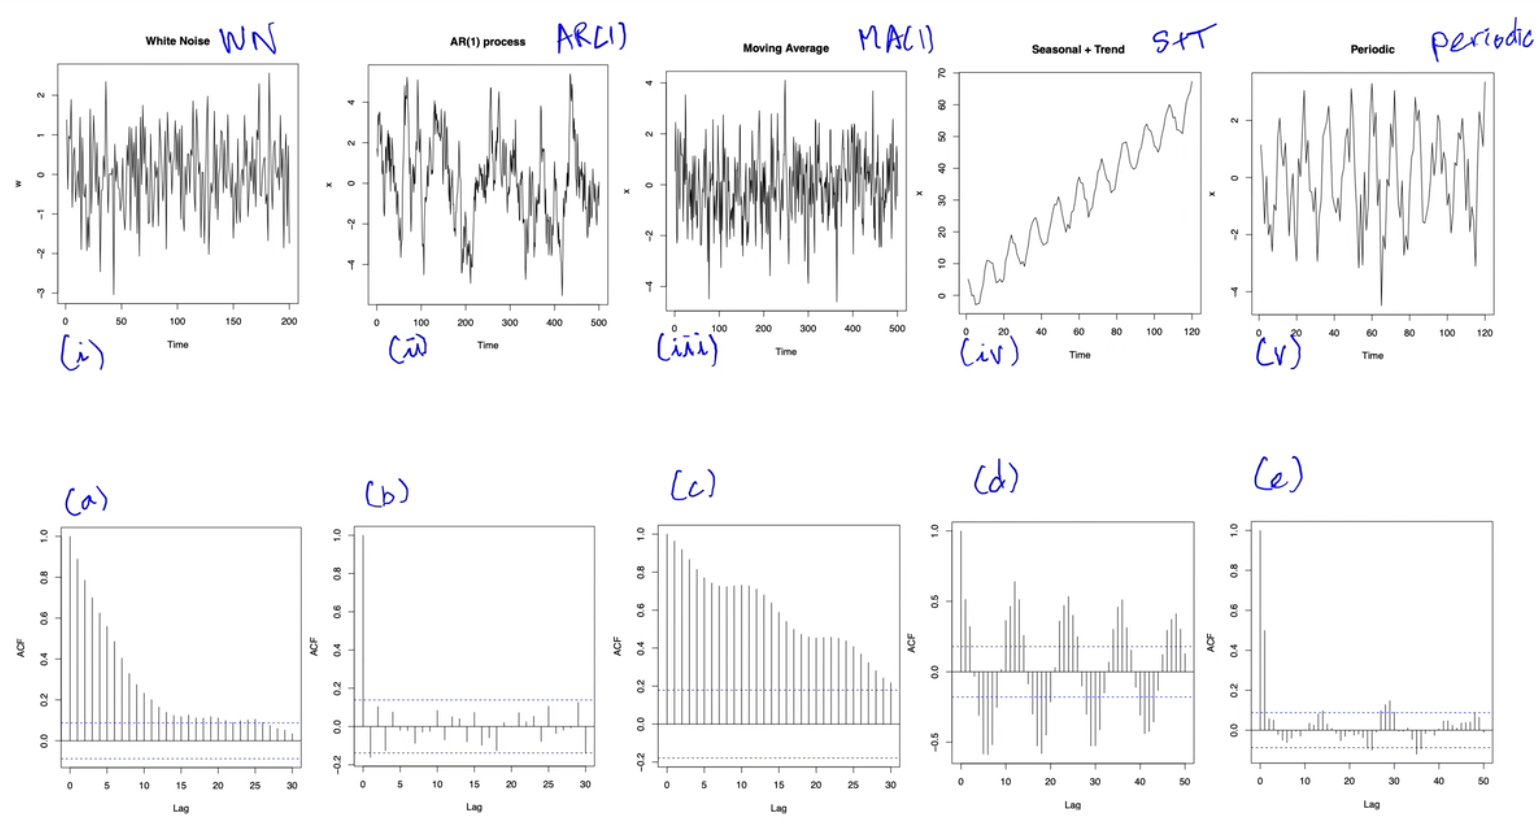
\includegraphics[width=14cm, height=10cm]{images/001_acf_match.png}
    \end{figure}
For White Noise process, everything should be uncorrelated except for $\rho(0)$, so the ACF should be plot b). \\
For AR(1) process, we have $\phi^{|h|}$, so it just decrease as $h$ increases. Hence it matches to a). \\
For MA(1) process, we have the autocorrelation to be 0 outside of the MA order, so it matches to e). \\
For seasonal + trend, we know that the trend will induce correlation at long lags, then we have periodic struction, hence c). \\
Finally periodic will have only periodic ACF. 

\section{ACF and Least Square Prediction}

\subsection{Primer with Gaussian Process}
Best LS estiamte of $x_{n+h}|x_n$: \\
Suppose $x=(x_1,...,x_{n+h})$ is jointly Gaussian, then we have 
    \begin{align*}
        f_x(x) = \frac{1}{(2\pi)^{\frac{n+h}{2}} |\Sigma|^{1/2}}e^{-\frac{1}{2}(x-\mu)^T\Sigma^{-1}(x-\mu)}
    \end{align*}
    \begin{itemize}
        \item $\Sigma$ matrix is a matrix with variance on the diagonal, and $cov(x_i, x_j)=\rho(i,j)*\sigma_i*\sigma_j$ on other entries.
    \end{itemize}
Given the jointly Gaussian, we have that the distribution of pair $(x_n, x_{n+h})$ is just a bivariate Gaussian distribution. i.e.: 
    \begin{align*}
        \begin{pmatrix}
            x_n \\ x_{n+h}
        \end{pmatrix} \sim 
        N \left ( 
            \begin{pmatrix}
            \mu_n \\ \mu_{n+h}
            \end{pmatrix}
            , 
            \begin{pmatrix}
            \sigma_n^2 & \rho(n, n+h)\sigma_n\sigma_{n+h} \\
            \rho(n, n+h)\sigma_n\sigma_{n+h} & \sigma_{n+h}^2
            \end{pmatrix}            
        \right )
    \end{align*}
The conditional distribution of $x_{n+h}|x_n$ is: 
    \begin{align*}
        N(\mu_{n+h} + \rho(n, n+h) \frac{\sigma_{n+h}}{\sigma_n} (x_n - \mu_n), \sigma_{n+h}^2(1-\rho(n, n+h)^2))
    \end{align*}

Hence, if $\{x_t\}$ is Gaussian and stationary, the best estiamte of $x_{n+h}$ given $x_n = c_n$ is the conditional mean, hence 
    \begin{align*}
        & \mu_{n+h} + \rho(n, n+h) \frac{\sigma_{n+h}}{\sigma_n} (x_n - \mu_n)\\
        & = \mu + \rho(h)(c_n - \mu_n)
    \end{align*}
    \begin{itemize}
        \item $\rho(n, n+h) = \rho(h)$ due to stationarity 
        \item $\frac{\sigma_{n+h}}{\sigma_n} = 1$ due to variance being time insensitive. 
    \end{itemize}
and the MSE is 
    \begin{align*}
        E[(x_{n+h} - f(x_n))^2] 
        & =  E[(x_{n+h} - E[x_{n+h}|x_n])^2 |x_n] \\
        & = Var(x_{n+h}|x_n)
    \end{align*}
So notice that 
    \begin{itemize}
        \item predictive accuracy improves as $|\rho(h)|\rightarrow 1$
        \item prediction is linear in $x$
    \end{itemize}
    
\subsection{General Linear Prediction}
Goal: Predicting $x_{n+h}|x_n = c_n$ with $f(x_n)=a(x_n-\mu)+b$. Assume $\{x_t\}$ stationary with $E[x_t]=\mu$ and $var(x_t)=\sigma^2$. The best linear predictor has the form 
    \begin{align*}
        f(x_n) = \rho(h) (x_n - \mu) + \mu
    \end{align*}
and the MSE is 
    \begin{align*}
        \sigma^2(1 - \rho(h)^2)
    \end{align*}